\subsection{GraphGPS with HIG}
GraphGPS is by design a highly malleable model, which allows for easy additions to the code. Thus we decided to implement HIG-GraphClassification in GraphGPS, to combine two already existing papers. For this combination we specifically targeted the Positional Encodings \ref{fig:gps-hig-position}

\begin{figure}[ht]
    \centering
    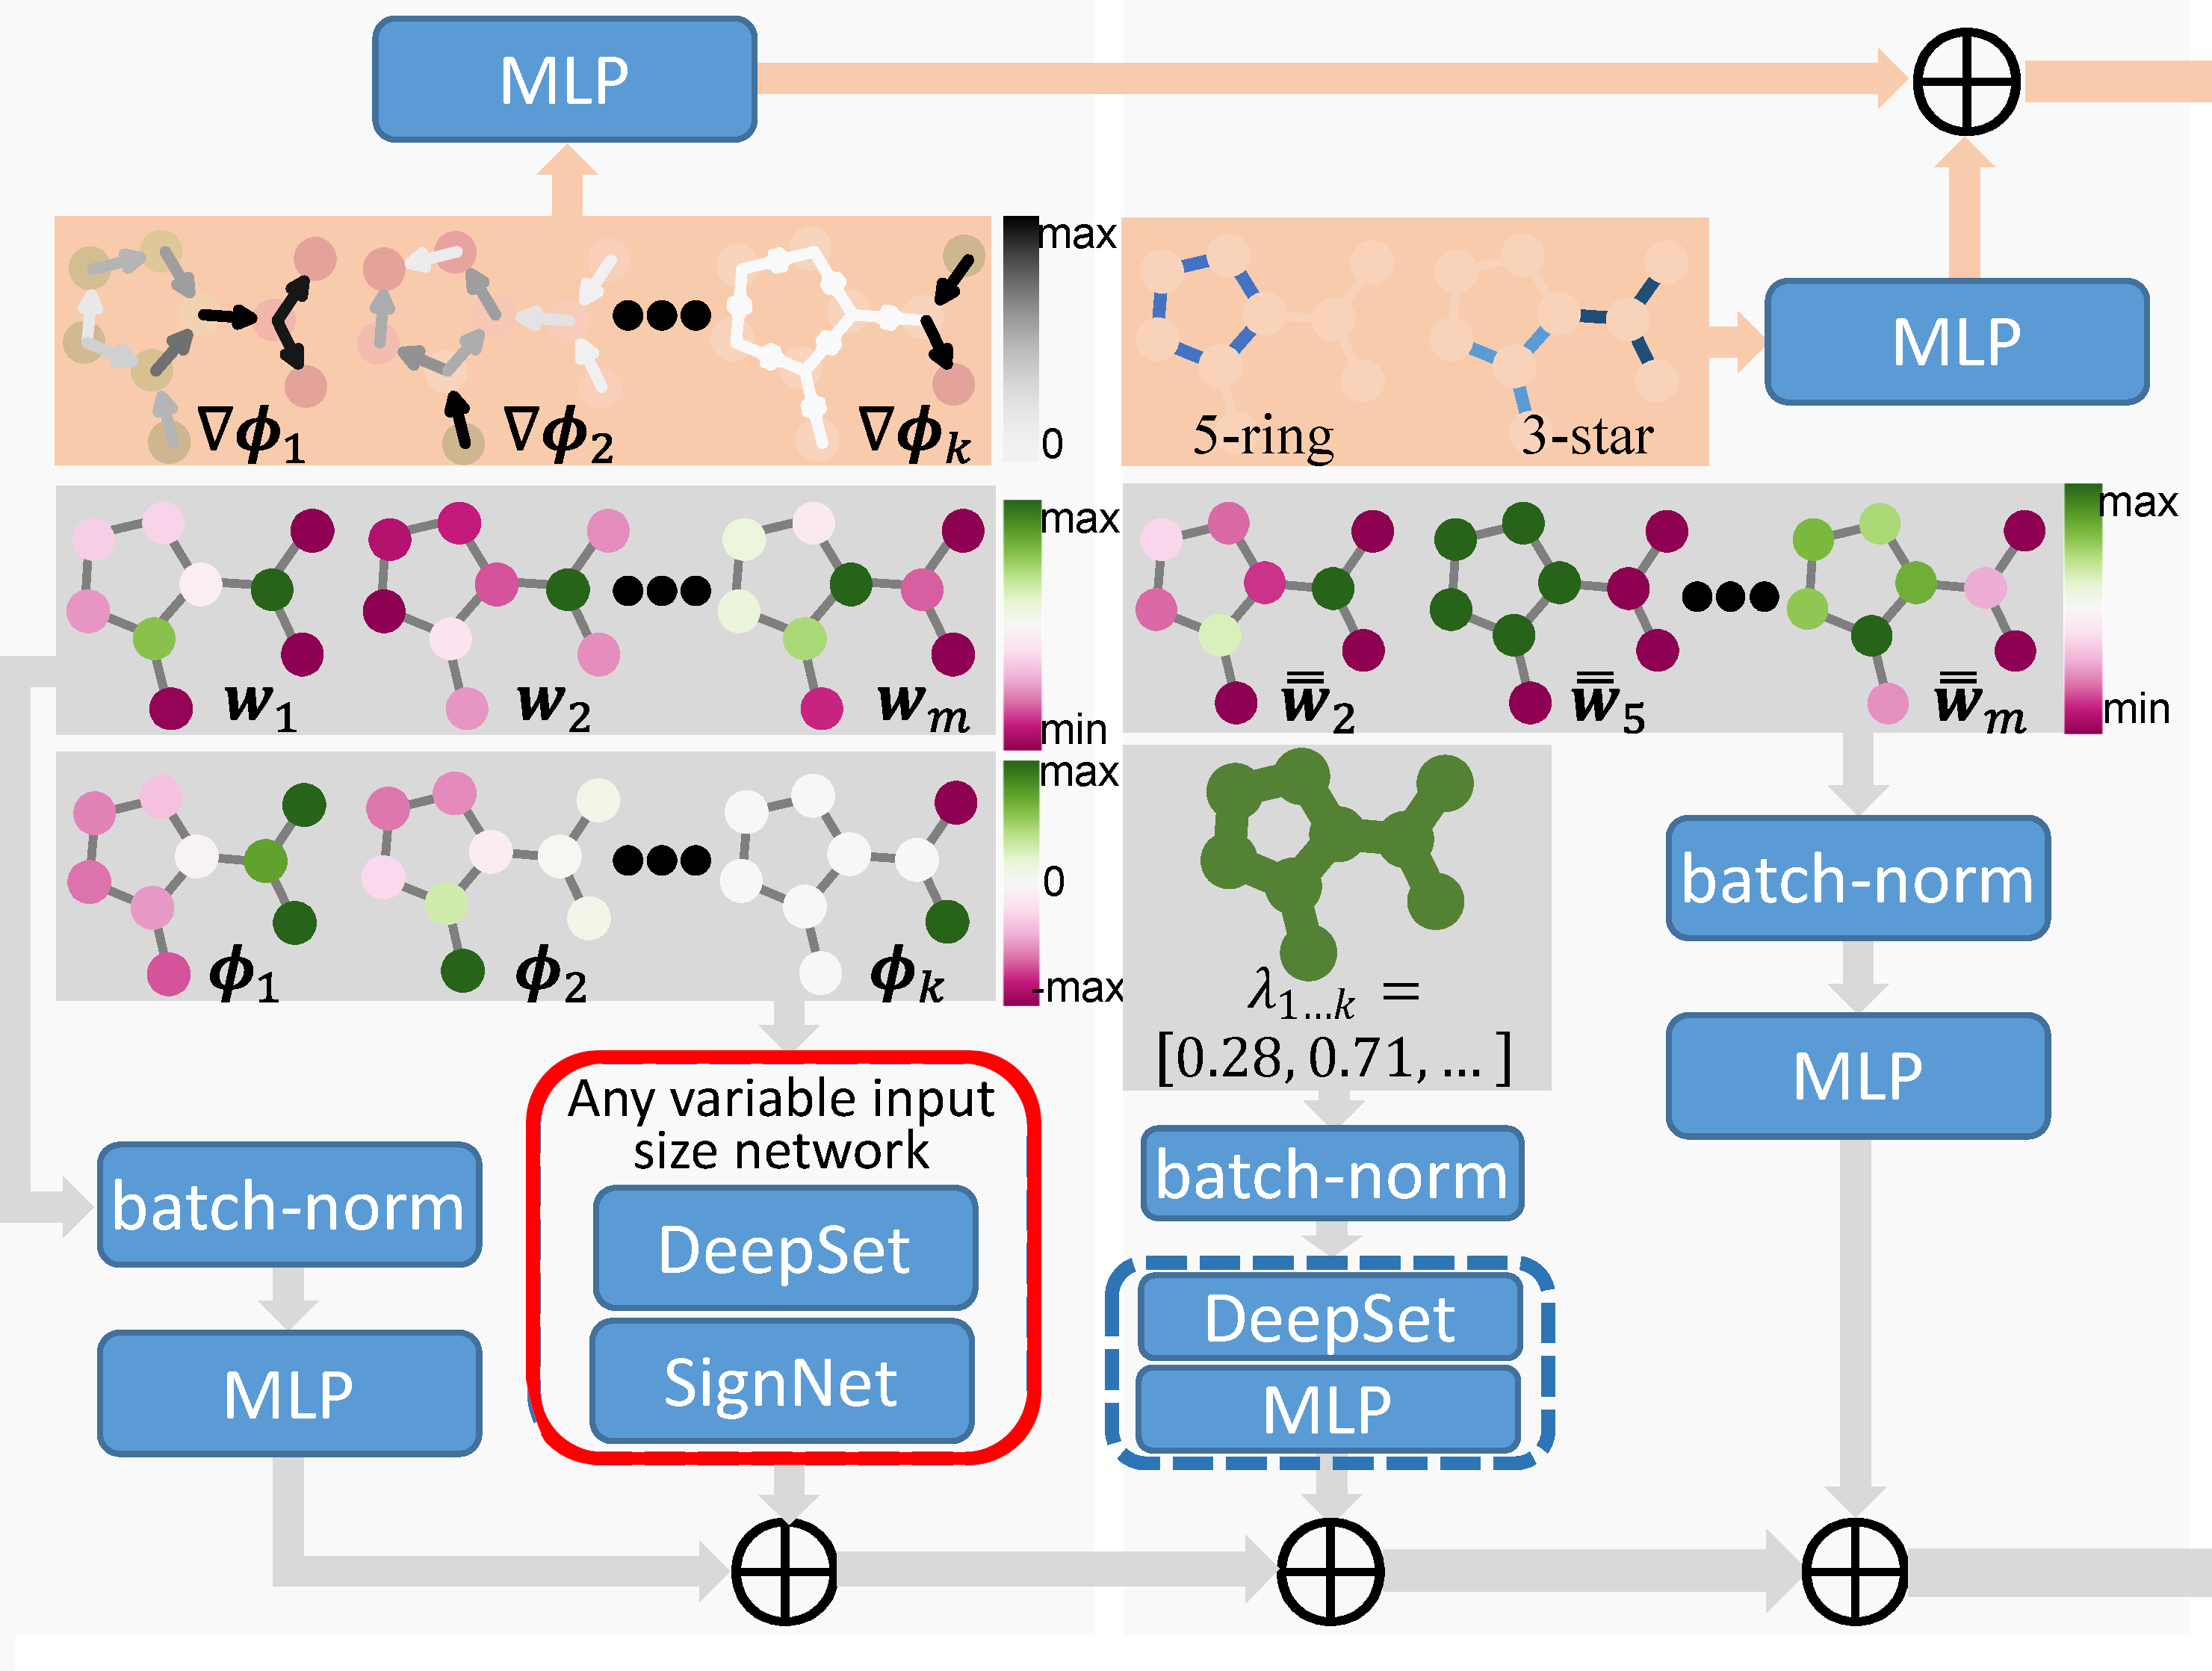
\includegraphics[scale=0.2]{tex/res/gps_hig_position.png}
    \caption{Position of HIG in GraphGPS structure}
    \label{fig:gps-hig-position}
\end{figure}

\subsubsection{Implementation}

The implementation of the heterogeneous interpolation, which involves dropping the feature vector of several randomly selected nodes and replacing them with an interpolated feature mix, can be found in algorithm \ref{algorithm:HiG_Code_in_GraphGPS}. While our implementation does not include the mixing ratio, we have added a Interpolation-p parameter and a min\_size parameter. The Interpolation-p parameter enables us to specify the probability with which the graph replaces a node with an interpolated feature mix. On the other hand, the min\_size parameter sets a minimum size for the graph. This is because a smaller graph tends to lose more information if a node is replaced, which could be disadvantageous. Additionally, we have included the nodes\_interpolated parameter, which allows us to specify the number of nodes that get dropped instead of randomly choosing how many get dropped.

\begin{minipage}{\linewidth}
    \begin{algorithm}[H]
        %\SetKwSty{text}
        \DontPrintSemicolon
        \SetArgSty{text}
        \SetProgSty{text}
        \SetKw{KwIn}{in}
        \SetKw{KwAnd}{and}

        \SetKwProg{Fn}{def}{}{}
        \If{'HiG' in pe\_types}{
            interpolation\_chance = cfg.posenc\_HIG.Interpolation-p\;
                is\_interpolating = np.random.choice(2, 1, p=[1-interpolation\_chance, interpolation\_chance])[0]\; 
                minimum\_node\_size = cfg.posenc\_HIG.minimum\_node\_size\;
                nodes\_interpolated = cfg.posenc\_HIG.nodes\_interpolated\;
                minimum\_node\_size = max(minimum\_node\_size, nodes\_interpolated)\;
            \If{data.num\_nodes > minimum\_node\_size \KwAnd is\_interpolating == 1}{
                rand\_ints = np.random.choice(data.num\_nodes, nodes\_interpolated\;
                sum = \{\}\;
                \For{rand\_int \KwIn rand\_ints}{
                data.x[rand\_int] = 0\;
                sum[rand\_int] = 0\;
            }
                \For{i \KwIn data.edge\_index[0]}{
                    \If{i \KwIn rand\_ints}{
                    relevant\_node = data.edge\_index[1][i]\;
                    data.x[i] = torch.add(data.x[i], data.x[relevant\_node])\;
                    sum[i] += 1\;
                    }
                }
                \For{rand\_int \KwIn rand\_ints}{
                data.x[rand\_int] = data.x[rand\_int] / sum[rand\_int]
            }
            }
        }
        \caption{HiG-Code in GraphGPS}
        \label{algorithm:HiG_Code_in_GraphGPS}
    \end{algorithm}
\end{minipage}

\subsubsection{Results on ogbg-molhiv}
In table \ref{hig_results} are the results of implementing HIG in GraphGPS. The lowest performance is when 5 nodes are replaced by an interpolation. GraphGPS with HIG performs best when combined with LapPE\cite{2023graphgps}. Without other Encodings the Parameter combination of 0.75 Interpolation-p, 1 Node Interpolated and 20 minimum graph Size performs best.
\begin{table}[ht!]
    \centering
    \caption{Results for different HIG Parameters}
    \label{hig_results}
    \begin{tabular}{c || l|l|l| p{6cm} |}
        Model Focus            & Interpolation-p & Nodes Interpolated & min.graph size & Test-AUC \\
        \hline
        \hline
        No HIG    &     &    &               &  0.7710  \\
        \hline
        Standard HIG      &  1.0& 1& 5            & 0.75274  \\
        \hline
        Interpolation-p               & 0.5& 1& 5                    & 0.77894  \\
                           & 0.1& 1& 5                    & 0.77033  \\
                           & 0.01& 1& 5                   & 0.7625   \\
        \hline
        Nodes Interpolated & 1.0& 2& 5                      & 0.73967  \\
                 & 1.0& 3& 5                      & 0.73882  \\
                                   & 1.0& 5& 10                      & 0.71498  \\
        \hline
        min. graph size    & 1.0& 1& 10                & 0.76795  \\
                 & 1.0& 1& 20                & 0.77084  \\
                           & 1.0& 1& 50                & 0.7566   \\
        \hline
        Combination   & 0.5& 1& 20                & 0.77164  \\
            & 0.75& 1& 20                & 0.78321  \\
        \hline
        HIG + RWSE   & 0.75& 1& 20                & 0.77924  \\
        \hline
        HIG + LapPE   & 0.75& 1& 20                & 0.78412  \\
    \end{tabular}
\end{table}


